\documentclass{article}

% Language setting
% Replace `english' with e.g. `spanish' to change the document language
\usepackage[english]{babel}

% Set page size and margins
% Replace `letterpaper' with `a4paper' for UK/EU standard size
\usepackage[letterpaper,top=2cm,bottom=2cm,left=3cm,right=3cm,marginparwidth=1.75cm]{geometry}

% Useful packages
\usepackage{amsmath}
\usepackage{graphicx}
\usepackage[colorlinks=true, allcolors=blue]{hyperref}

\title{HW7}
\author{irene0613}

\begin{document}
\maketitle


\section{Introduction}
  
\qquad This assignment involves using LoRA (Low-Rank Adaptation) and other Parameter Efficient Fine-Tuning (PEFT) methods to fine-tune a DistilBERT model for sequence classification on the IMDB dataset. The objective is to experiment with different method configurations and observe their results. 

\quad Detailed documentation is provided in the README.md file and the Transformers\_peft.ipynb notebook, along with screenshots of the training process conducted on Google Colab.

\section{Training Method}

\subsection{Model and Tokenizer}

\qquad We utilize \textbf{distilbert-base-cased} as our foundational model and ensure consistent initialization of the tokenizer from the model checkpoint.

\subsection{Data Preparation}

\begin{itemize}
    \item Load the IMDB movie review dataset using the  \textbf{datasets} library. The dataset contains 50,000 movie reviews labeled as positive or negative.
    \item Create a small-scale training and validation dataset from the IMDB dataset (ratio 4:1) and truncate each review to the first 50 tokens.
    \item Tokenize the newly created small-scale training and validation datasets in batches, processing 16 samples at a time.
\end{itemize}

\subsection{Training Parameters}

\begin{itemize}
    \item Batch Size: During each iteration, the model calculates the loss for this batch of data and updates the weights based on this loss. The choice of batch size affects training speed and model performance.
    \item Learning Rate: Controls the step size of model weight updates. It is a crucial parameter that influences the convergence speed and effectiveness during the training process.
    \item Evaluation Strategy: Ensures that the model does not overfit or underfit during training and provides immediate feedback to adjust training parameters. In this assignment, evaluation is done per epoch—after training one epoch, an evaluation is performed.
    \item Number of Epochs: Controls the number of times the model trains on the training dataset, ensuring the model has enough opportunities to learn patterns in the data.
\end{itemize}

\subsection{Trainer}

\qquad The Hugging Face Trainer manages the training process and is responsible for model initialization, training parameter settings, setup of training and validation datasets, tokenizer configuration, and custom evaluation metrics.

\subsection{LoRA \& IA3 Configurations and Their Corresponding Results}

\begin{itemize}
    \item LoraConfig\_1
    \begin{verbatim}
    peft_config_1 = LoraConfig(
        lora_alpha=16,          
        lora_dropout=0.1,         
        r=64,              
        bias="none",          
        task_type="SEQ_CLS",      
        target_modules=["q_lin", "v_lin", "k_lin", "out_lin"], 
    )
    \end{verbatim}
    \begin{figure}[h]
    \centering
    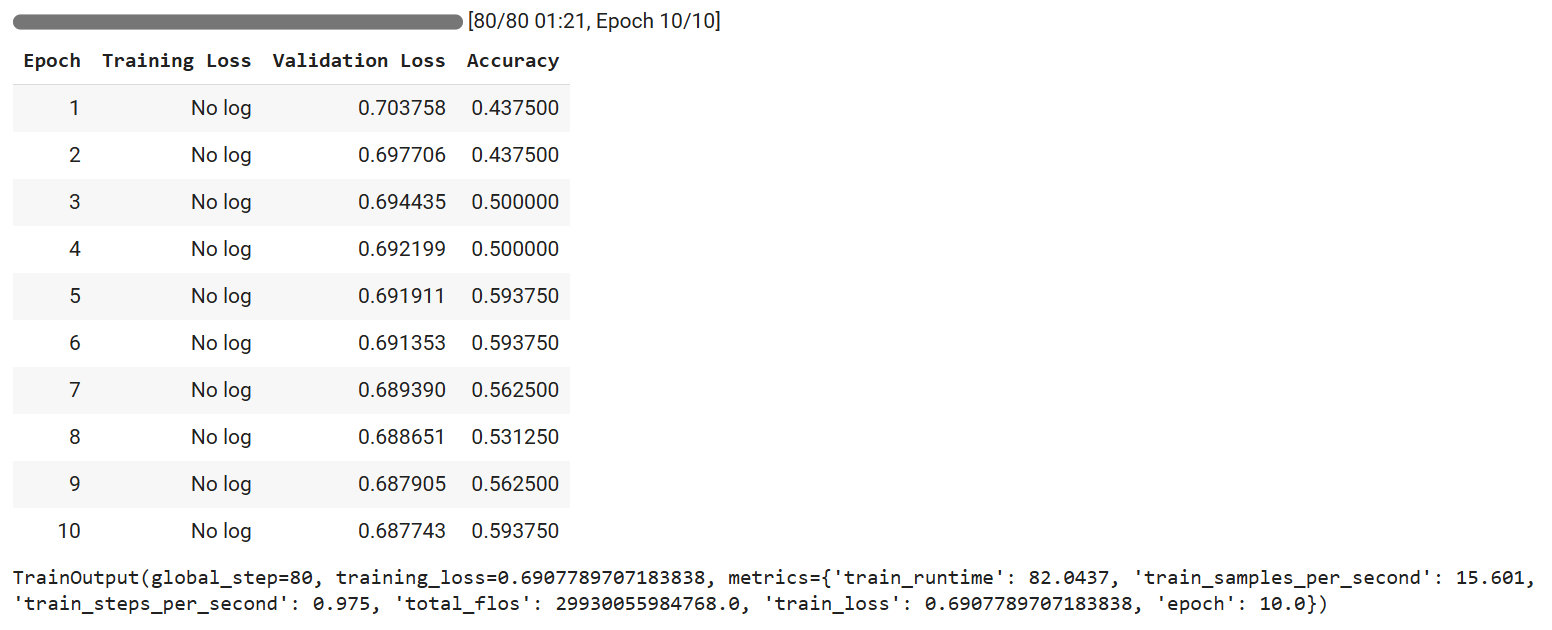
\includegraphics[width=0.6\textwidth]{lora_1.png}
    \caption{Training result LoraConfig\_1}
    \label{fig:lora_1}
    \end{figure}
        
    \item LoraConfig\_2
    \begin{verbatim}
    peft_config_2 = LoraConfig(
        lora_alpha=16,
        lora_dropout=0.1,
        r=64,
        bias="none",
        task_type="SEQ_CLS",
        target_modules=["q_lin", "v_lin", "k_lin", "out_lin", "ffn.lin1", "ffn.lin2"],  
    )
    \end{verbatim}
    \begin{figure}[h]
    \centering
    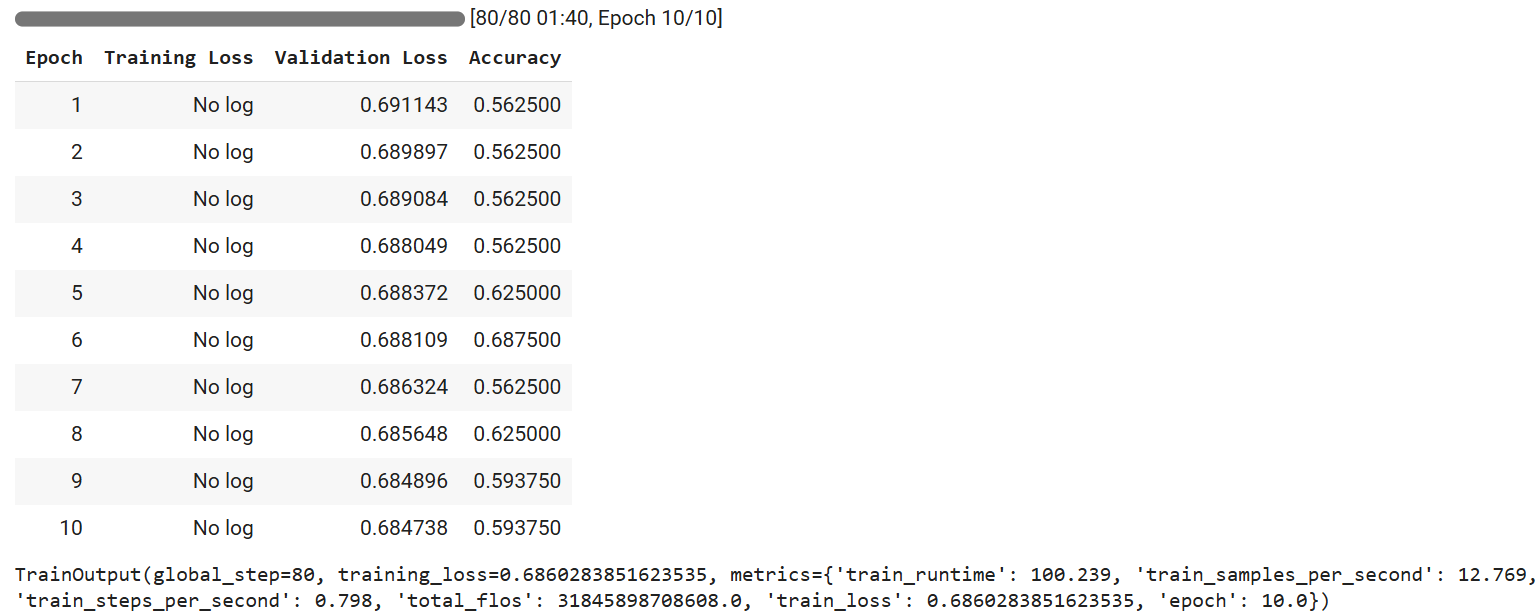
\includegraphics[width=0.6\textwidth]{lora_2.png}
    \caption{Training result LoraConfig\_2}
    \label{fig:lora_2}
    \end{figure}

    \vspace{70pt}
    \item LoraConfig\_3
    \begin{verbatim}
    peft_config_3 = LoraConfig(
        lora_alpha=32,
        lora_dropout=0.2,
        r=32,
        bias="none",
        task_type="SEQ_CLS",
        target_modules=["q_lin", "v_lin", "k_lin", "out_lin"],
    )
    \end{verbatim}
    \begin{figure}[h]
    \centering
    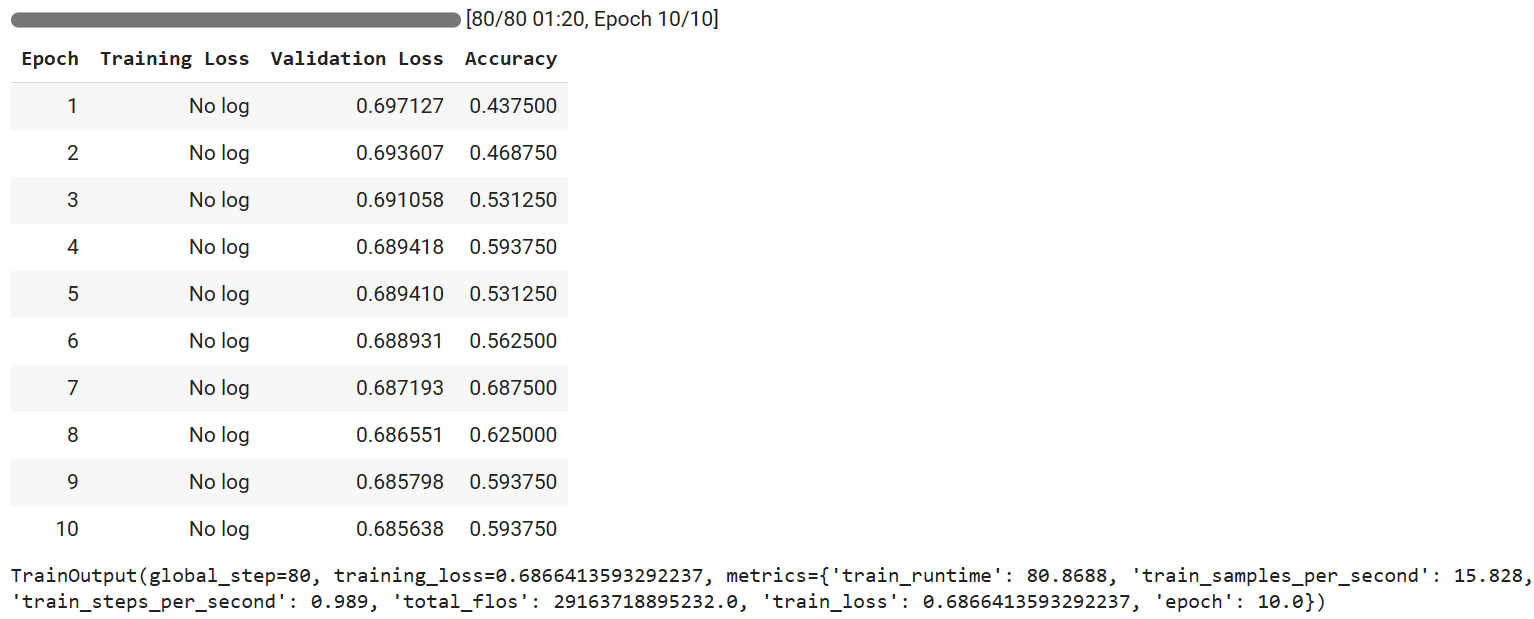
\includegraphics[width=0.6\textwidth]{lora_3.png}
    \caption{Training result LoraConfig\_3}
    \label{fig:lora_3}
    \end{figure}
    
    \item IA3Config
    \begin{verbatim}
    peft_config_4 = IA3Config(
        task_type=TaskType.SEQ_CLS,
        target_modules=["q_lin", "v_lin", "k_lin", "out_lin", "ffn.lin1", "ffn.lin2"],
        feedforward_modules=["ffn.lin1", "ffn.lin2"],
    )
    \end{verbatim}
    \begin{figure}[h]
    \centering
    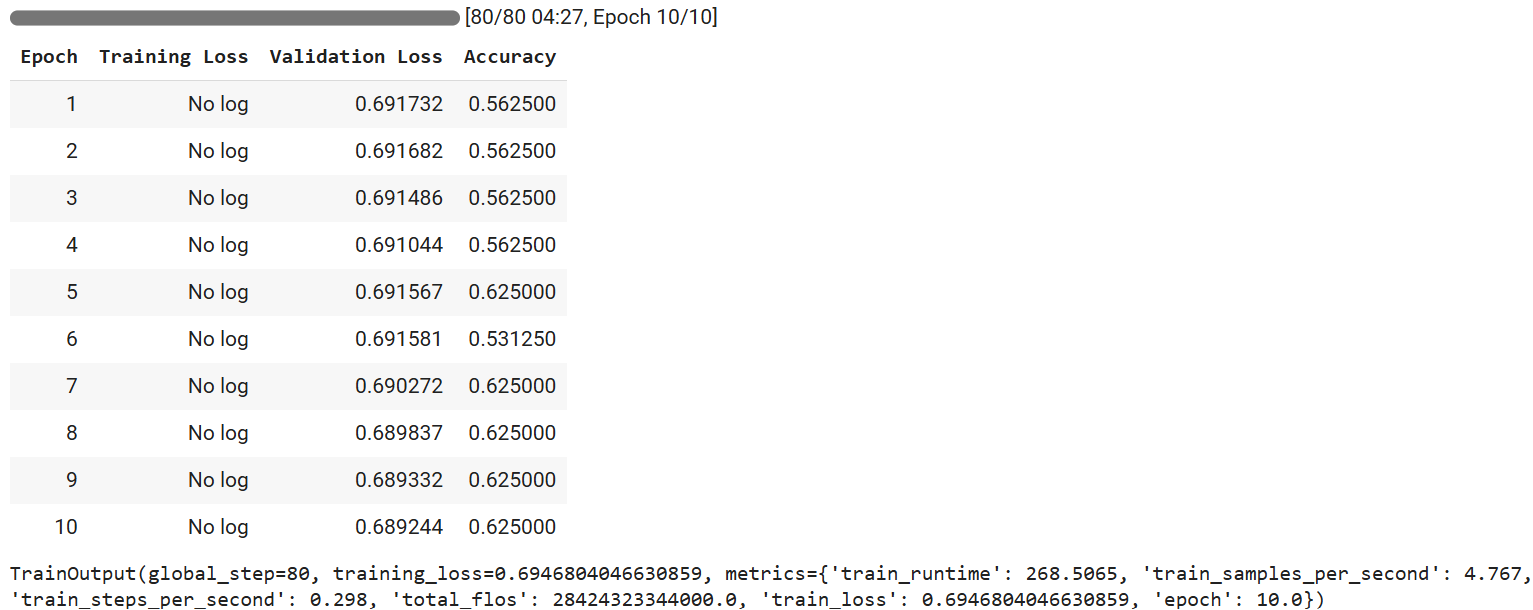
\includegraphics[width=0.6\textwidth]{IA3.png}
    \caption{Training result IA3Config}
    \label{fig:IA3}
    \end{figure}
    
\end{itemize}





\end{document}